\subsection*{The Division Algorithm}
\index{Division Algorithm|(}%
\typeu Activity~\ref*{PA:quotients} was an introduction to a mathematical result known as the Division Algorithm.  One of the purposes of this \typel activity was to illustrate that we have already worked with this result, perhaps without knowing its name.  For example, when we divide 337 by 6, we often write
\[
\frac{{337}}{6} = 56 + \frac{1}{6}.
\]
When we multiply both sides of this equation by 6, we get
\[
337 = 6 \cdot 56 + 1.
\]
When we are working within the system of integers, the second equation is preferred over the first since the second one uses only integers and the operations of addition and multiplication, and the integers are closed under addition and multiplication.  Following is a complete statement of the Division Algorithm.
%\hbreak
%
\begin{flushleft}\label{divalgorithm}
\fbox{\parbox{4.68in}{
\textbf{The Division Algorithm} \\
For all integers $a$ and $b$ with $b>0$,  there exist unique integers $q$ and $r$ such that
\[
a=bq+r  \text{ and }  0 \leq r < b.
\]
}}
\end{flushleft}

%\begin{divalgo}\label{T:divalgo} \hfill

%\noindent
%Let  $a$, $b$, and  $c$  be integers with $b>0$.  Then, there exist unique integers $q$ and $r$ %such that
%\[
%a=bq+r  \text{ and }  0 \leq r < b.
%\]
%\end{divalgo}
%

%\begin{flushleft}
\noindent
\textbf{Some Comments about the Division Algorithm}
\begin{enumerate}
\item The Division Algorithm can be proven, but we have not yet studied the methods that are usually used to do so.  In this text, we will treat the Division Algorithm as an axiom of the integers.  The work in  \typeu Activity~\ref*{PA:quotients} provides some rationale that this is a reasonable axiom.

\item The statement of the Division Algorithm contains the new phrase, ``there exist unique integers $q$  and  $r$  such that $ \ldots .$''   This means that there is only one pair of integers  $q$  and  $r$  that satisfy both the conditions  $a = bq + r$ and 
$0 \leq r < b$.  As we saw in \typeu Activity~\ref*{PA:quotients}, there are several different ways to write the integer  $a$  in the form  $a = bq + r$.  However, there is only one way to do this and satisfy the additional condition that  $0 \leq r < b$.

\item In light of the previous comment, when we speak of \textbf{the quotient}
\index{quotient}%
 and \textbf{the remainder}
\index{remainder}%
 when we ``divide an integer  $a$  by the positive integer  $b$,'' we will always mean the quotient $\left( q \right)$  and the remainder  $\left( r \right)$ guaranteed by the Division Algorithm.  So the remainder $r$ is the least nonnegative integer such that there exists an integer (quotient) $q$ with $a = bq + r$.

\item If  $a < 0$, then we must be careful when writing the result of the Division Algorithm.  For example, in parts~(\ref{PA:quotients4}) and~(\ref{PA:quotients5}) of \typeu Activity~\ref*{PA:quotients}, with $a =  - 17$  and  
$b = 5$, we obtained $-17 = 5\cdot(-4) + 3$, and so the quotient is $-4$ and the remainder is 3.  Notice that this is different than the result from a calculator, which would be $\dfrac{{ - 17}}{5} =  - 3.4$.  But this means
\[
\frac{{ - 17}}{5} =  - \left( {3 + \frac{4}{{10}}} \right) =  - 3 - \frac{2}{5}.
\]
If we multiply both sides of this equation by 5, we obtain
\[
{-17} = 5\left( { - 3} \right) + \left( { - 2} \right).
\]
This is not the result guaranteed by the Division Algorithm since the value of $-2$ does not satisfy the result of being greater than or equal to 0 and less than 5.  


\item One way to look at the Division Algorithm is that the integer  $a$  is either going to be a multiple of  $b$, or it will lie between two multiples of  $b$.  Suppose that  $a$  is not a multiple of  $b$ and that it lies between the multiples  $b \cdot q$  and  $b\left( {q + 1} \right)$, where $q$ is some integer.  This is shown on the number line in Figure~\ref{fig:divalgo}.
%
\begin{figure}[h]
\begin{center}
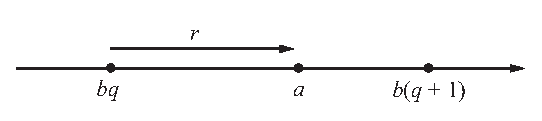
\includegraphics{figps-divalgo.eps}
\caption{Remainder for the Division Algorithm}\label{fig:divalgo}
\end{center}
\end{figure}

If  $r$  represents the distance from  $b \cdot q$ to  $a$, then
\[
\begin{aligned}
  r &= a - b \cdot q,\text{ or} \\ 
  a &= b \cdot q + r. \\ 
\end{aligned} 
\]
From the diagram, also notice that  $r$  is less than the distance between  $b \cdot q$
  and  $b\left( {q + 1} \right)$.  Algebraically, this distance is
\[
\begin{aligned}
  b\left( {q + 1} \right) - b \cdot q &= b \cdot q + b - b \cdot q \\ 
                                      &= b. \\ 
\end{aligned} 
\]
Thus, in the case where  $a$  is not a multiple of  $b$, we get  $0 < r < b$.

\item We have been implicitly using the fact that an integer cannot be both even and odd.  There are several ways to understand this fact, but one way is through the Division Algorithm.  When we classify an integer as even or odd, we are doing so on the basis of the remainder (according to the Division Algorithm) when the integer is ``divided'' by 2.  If  $a \in \mathbb{Z}$, then by the Division Algorithm there exist unique integers  $q$  and  $r$  such that
\[
a = 2q + r\text{  and  }0 \leq r < 2.
\]
This means that the remainder, $r$,  can only be zero or one (and not both).  When  $r = 0$, the integer is even, and when  $r = 1$, the integer is odd.
\end{enumerate}
\index{Division Algorithm|)}%
\vskip3pt
\hrule
%\pagebreak
%\hbreak

\begin{prog}[\textbf{Using the Division Algorithm}]\label{pr:usingdivalgo} \hfill 
\begin{enumerate}

\item What are the possible remainders (according to the Division Algorithm) when an integer is
\begin{multicols}{2}
\begin{enumerate}
\item Divided by 4?
\item Divided by 9?
\end{enumerate}
\end{multicols}

\item For each of the following, find the quotient and remainder (guaranteed by the Division Algorithm) and then summarize the results by writing an equation of the form $a = bq + r$, where 
$0 \leq r < b$.

\begin{multicols}{2}
\begin{enumerate}
\item When 17 is divided by 3.
\item When $-17$ is divided by 3.
\item When 73 is divided by 7.
\item When $-73$ is divided by 7.
\item When 436 is divided by 27.
\item When 539 is divided by 110.
\end{enumerate}
\end{multicols}
\end{enumerate}
\end{prog}
\hbreak

\endinput
